\chapter{Lec 09-10 - Regularization}

\section{Regularization}
Neural networks are usually \textit{over-parameterized}, that is, they have more parameters than training examples. This implies that the set of parameters can perfectly fit the training data, including the noise (overfitting). In order to limit overfitting, we can perform \textbf{regularization}, that is, any modification we make to a learning algorithm intended to reduce its generalization error but not its training error. Basically, regularization aims at reducing the \textbf{variance} error (favour simpler hypothesis).\newline\newline
Oldest regularization strategies (adopted for linear/logistic regression) limit the capacity of the models, adding a parameter \textbf{norm penalty} to the \textbf{objective function}
\[\tilde{J}(\theta; \textbf{X}; \textbf{y}) = J(\theta; \textbf{X}; \textbf{y}) + \alpha \Omega(\theta)\]
where $\Omega$ is the so called \textbf{regularization term} that depends on the model's parameters. Larger values of the hyper-parameter $\alpha$ results in more regularization. This is because if $\alpha$ is very high, the optimization will favour the second term more than the first and viceversa. In general, only weights are regularized (bias terms tend to be easy to learn).
\begin{center}
    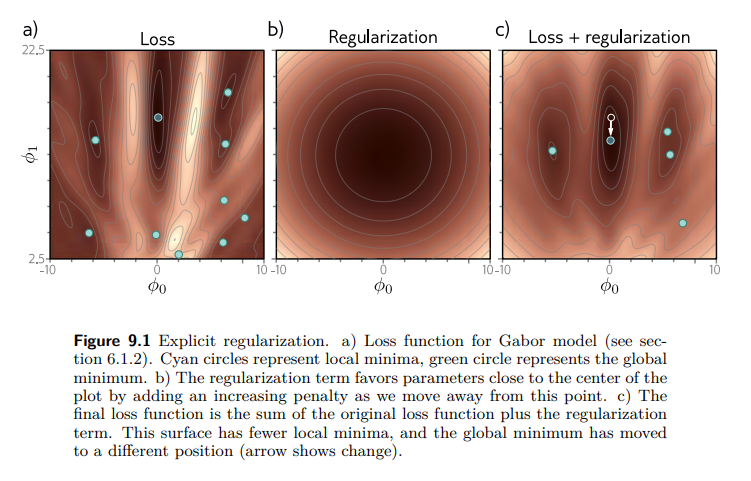
\includegraphics[]{images/Reg.png}
\end{center}
How can we set this regularization term?

\section{Weight decay ($L^2$ norm)}
The idea is to drive the weights close to the origin:
\[\Omega(\theta) = \frac{1}{2} ||w||_2^2\]
where $||w||_2^2$ is the 2-norm of the weight vector ($w^Tw$).\newline\newline
So our new cost function will become:
\[\tilde{J}(\textbf{w}; \textbf{X}, \textbf{y}) = \frac{\alpha}{2}\textbf{w}^T\textbf{w} + J(\textbf{w}; \textbf{X}, \textbf{y})\]
Note that, for simplicity, we are assuming no bias.\newline\newline
Then, we have to compute the gradient of the new cost function with respect to $\textbf{w}$:
\[\nabla_\textbf{w} \tilde{J}(\textbf{w}; \textbf{X}, \textbf{y}) = \alpha \textbf{w} + \nabla_\textbf{w} J(\textbf{w}; \textbf{X}, \textbf{y})\]
A single step of stochastic gradient descent with learning rate $\epsilon$ would be:
\[\textbf{w} \gets \textbf{w} - \epsilon(\alpha \textbf{w} + \nabla_\textbf{w} J(\textbf{w}; \textbf{X}, \textbf{y}))\]
\[\textbf{w} \gets (1 - \epsilon\alpha)\textbf{w} - \epsilon \nabla_\textbf{w} J(\textbf{w}; \textbf{X}, \textbf{y})\]
Basically, we are multiplying the weights vector for a value strictly smaller than 1, so it becomes smaller every SGD step. The weights get shrinked on each step (weight decay). This approach is based on the fact that large weights lead to amplifications of the differences between similar inputs, making the network sensitive, and hence overfitting, to its training data. In contrast, small weights reduce the differences between similar inputs, and hence provides improved generalization.

\subsection{Ordinary Least squares}
Regularization is necessary in some ill-posed ML problems:
\begin{itemize}
    \item When we have less examples than features

    \item Or more in general when the solution is not unique
\end{itemize}
Let's consider linear regression:
\[\textbf{Xw} = \textbf{y}\]
Let's define MSE loss:
\[J(\textbf{w}) = \frac{1}{n}||\textbf{Xw} - \textbf{y}||^2\]
The gradient of $J$ with respect to $\textbf{w}$ is:
\[\nabla_\textbf{w}J = \frac{1}{n}2(\textbf{Xw} - \textbf{y})^T \textbf{X}\]
Now, we can define the closed-form solution equating the derivative to zero:
\[\begin{split}
    \frac{1}{n}2(\textbf{Xw} - \textbf{y})^T \textbf{X} = 0\\
    \textbf{w} = (\textbf{X}^T \textbf{X})^{-1}\textbf{X}^T\textbf{y}
\end{split}\]
Note that $(\textbf{X}^T \textbf{X})^{-1}$ should be invertible, that is, a square full-rank matrix. $\textbf{X}^T \textbf{X}$ is always square, but it is not invertible when the number of variables exceeds the number of data points.\newline\newline
With MSE loss and $L^2$ norm, the gradients would be:
\[\nabla_\textbf{w}J = 2(\textbf{Xw} - \textbf{y})^T \textbf{X} + 2\alpha \textbf{w}^T\]
Therefore, the closed-form solution will be:
\[\begin{split}
    2(\textbf{Xw} - \textbf{y})^T \textbf{X} + 2\alpha \textbf{w}^T = 0\\
    \textbf{w} = (\textbf{X}^T \textbf{X} + \alpha \textbf{I})^{-1}\textbf{X}^T \textbf{y}
\end{split}\]
$(\textbf{X}^T \textbf{X} + \alpha \textbf{I})^{-1}$ is a full-rank matrix and therefore always invertible. The diagonal entries of this matrix correspond to the variance of each input feature, and we add $\alpha$ on this diagonal. We can see that $L^2$ regularization causes the learning algorithm to “perceive” the input $\textbf{X}$ as having higher variance, which makes it shrink the weights on features whose covariance with the output target is low compared to this added variance.


\section{$L^1$ Regularization}
In $L^1$ regularization, $\Omega$ and $\tilde{J}$ are defined as follows:
\[\Omega(\theta) = ||w||_1\]
\[\tilde{J}(\textbf{w}; \textbf{X}, \textbf{y}) = \alpha ||w||_1 + J(\textbf{w}; \textbf{X}, \textbf{y})\]
With gradient $\nabla_\textbf{w}\tilde{J}(\textbf{w};\textbf{X}, \textbf{y}) = \alpha \, sign(\textbf{w}) + \nabla_\textbf{w}J(\textbf{w};\textbf{X}, \textbf{y})$ where $sign(\cdot)$ is applied element-wise. This technique forces the solution to be sparse (i.e. lot of weights to 0 and only few of them $\neq 0$). Therefore, it performs \textbf{feature selection}.\newline\newline
This sparsity property can be seen looking at the gradients formula:
\[\nabla_\textbf{w}\tilde{J}(\textbf{w};\textbf{X}, \textbf{y}) = \alpha \, sign(\textbf{w}) + \nabla_\textbf{w}J(\textbf{w};\textbf{X}, \textbf{y})\]
If $w_i$ is negative, then the term $\alpha \,sign(w_i)$ will be negative and viceversa. Therefore, when we'll perform the update by subtracting the gradients, $w_i$ will be pushed in the opposite direction of its sign by $\alpha$.

\subsection{Geometric interpretation}
Consider a linear regression:
\[\textbf{Xw} = \textbf{y}\]
Given an example in the training set, e.g. $([10, 1], 5)$, we have infinitely many solutions satisfying:
\[\begin{split}
    10 w_1 + w_2 = 5 \\
    w_2 = 5 - 10 w_1
\end{split}\]
\begin{center}
    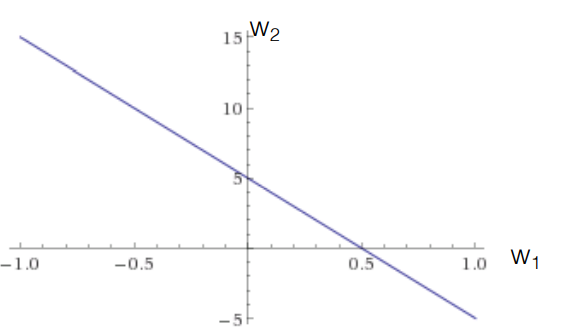
\includegraphics[scale=0.7]{images/geometric l1.png}
\end{center}
This family of solutions (which are infinite) lies on the blue line in the $w_1, w_2$ space represented in the figure above.\newline\newline
The $L^1$ norm is defined as the sum of absolute values:
\[||\textbf{w}||_1 = \sum_i |w_i|\]
In the $w_1, w_2$ space defined previously, all the points with constant $L^1$ norm $c$ lies on a square.
\begin{center}
    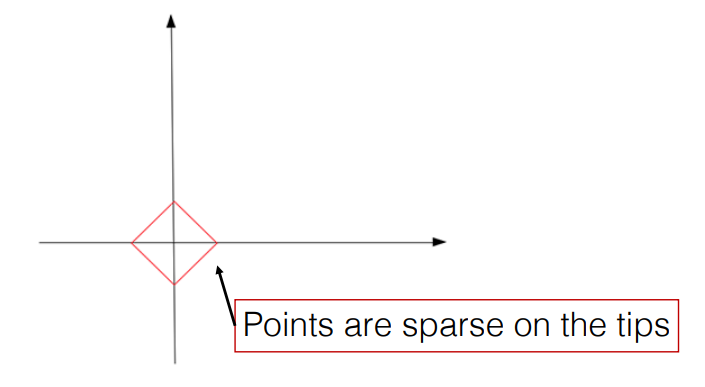
\includegraphics[scale=0.7]{images/l1 reg..png}
\end{center}
If we want to find the solution for $w_2 = 5 - 10 w_1$ with minimum $L^1$ norm, we have to look at the point where it intersects the square.
\begin{center}
    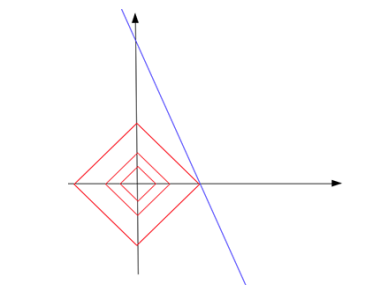
\includegraphics[scale=0.7]{images/l1 sparse.png}
\end{center}
This intersection will probably be on one of the axis, that is, the solution with minimum $L^1$ norm will \textbf{probably} be sparse. This is not always true, but in high-dimensional spaces it is likely.\newline\newline
In the case of $L^2$ norm, instead of a square, the points with constant norm will make a circle (in 2-dimensions). $L^2$ does not enforce sparsity because the solution with minimum norm can be at any point on the circle. Therefore,  $L^2$ causes all the weights to be shrunk towards zero, but none of them are driven to exactly zero.

\section{Data augmentation}
The idea of data augmentation is to generate \textit{fake} training data in order to enrich the training set. For example, in object detection on images, we want the model to be invariant to rotation, translation or scaling; therefore, we can apply some transformations on the training instances in order to achieve this goal.\newline\newline
Another way to perform data augmentation is to inject noise in:
\begin{itemize}
    \item the input examples (e.g. denoising autoencoders)
    \item the hidden representations (e.g. droput)
    \item the target (e.g. label smoothing). Consider a multi-class classification problem. Since the softmax will never give exactly 1 or 0, there will always be a gradient that makes the weights bigger. Label smoothing regularizes a model based on a softmax with $k$ output values by replacing the hard 0 and 1 classification targets with targets of $\frac{\epsilon}{k - 1}$ and $1 - \epsilon$, respectively.\newline\newline
    This technique is also useful if the dataset has some amount of mistakes in the $y$ labels.
\end{itemize}

\section{Semi-supervised learning}
Let's say that we have a problem for which it's easy to gather the data but it's very difficult to set labels for those data. In the paradigm of semi-supervised learning, both unlabeled examples from $P(\textbf{x})$ and labeled examples from $P(\textbf{x}, \textbf{y})$ are used to estimate $P(\textbf{y}|\textbf{x})$ or predict $\textbf{y}$ from
$\textbf{x}$.\newline\newline
We learn a representation $h = f(\textbf{x})$ such that similar examples are close in the new space. A linear classifier in the new space may achieve better generalization. Unsupervised learning can provide useful cues for how to group examples in representation
space.\newline\newline
Instead of having separate unsupervised and supervised components in the model, one can construct models in which a generative model of $P(\textbf{x})$ (autoencoder) shares parameters with a discriminative model of $P(\textbf{y} | \textbf{x})$.

\section{Transfer learning}
When training data is limited, other datasets can be exploited to improve performance. Transfer learning means transferring information from previously learned tasks for the learning of new tasks. Basically, we can take a model that was trained on a similar task and adapt it to our problem. In the case of Neural Networks, we can do this by removing the last layer of the network and adding one or more layers in order to produce a suitable output. The main model may be fixed and the new layers trained for the new task, or we may fine-tune the entire model.\newline\newline
Transfer learning can be viewed as initializing most of the weights of the final network in a sensible part of the space that is likely to produce a good solution.

\section{Multi-Task learning}
Multi-task learning (MTL) is a subfield of machine learning in which multiple learning tasks are solved at the same time. Part of the model is shared across different tasks, and is driven to learn a representation that generalizes well.

\section{Self-supervised learning}
When no data from other tasks is available, we can create large amounts of \textit{free} labeled data using self-supervised learning and use this for transfer learning. For example:
\begin{itemize}
    \item \textbf{generative} self-supervised learning: part of each data example is masked and the learning task is to predict the missing part.

    \item \textbf{contrastive} self-supervised learning: two versions of each unlabeled example are presented, when one has been distorted in some way. The system is trained to predict which is the original.
\end{itemize}

\section{Early stopping}
When training large models with sufficient representational capacity to overfit
the task, we often observe that training error decreases steadily over time, but
validation set error begins to rise again. This means we can obtain a model with better validation set error (and thus, hopefully, better test set error) by returning the model's parameters at the point in time with the lowest validation set error. When the training algorithm terminates, we return these parameters, rather than the latest parameters. The training algorithm terminates when no parameters have improved over the best recorded validation error for some pre-specified number of iterations.\newline\newline
Early stopping acts as a regularizer because it has the effect of
restricting the optimization procedure to a relatively small volume of parameter space in the neighborhood of the initial parameter values.

\section{Parameter Tying and sharing}
Sometimes we might not know precisely what values the parameters should take but we know, from knowledge of the domain and model architecture, that there should be some dependencies between the model parameters.\newline\newline
A common type of dependency that we often want to express is that certain parameters should be close to one another. Consider the following scenario: we have two models performing the same classification task (with the same set of classes) but with somewhat different input distributions. Let us imagine that the tasks are similar enough that we believe the model parameters should be close to each other. We can leverage this information
through regularization. Specifically, we can use a parameter norm penalty of the form:
\[\Theta (w^{(A)}, w^{(B)}) = ||w^{(A)} - w{(B)}||^2_2\]
Basically, it is a regularization term penalizing distant parameters. While a parameter norm penalty is one way to regularize parameters to be close to one another, the more popular way is to use constraints: to force sets of parameters to be equal. This method of regularization is often referred to as
\textbf{parameter sharing}, because we interpret the various models or model components as sharing a unique set of parameters.\newline\newline
By far the most popular and extensive use of parameter sharing occurs in convolutional neural networks (CNNs) applied to computer vision. The same feature is computed over different locations in the input. This means that we can find a cat with the same cat detector whether the cat appears at column $i$ or column $i + 1$ in the image.

\section{Sparse representation}
We have seen $L^1$ regularization to induce weight sparsity. We can similarly induce \textbf{representation sparsity} by placing a penalty on the activations of the units in a neural network, encouraging their activations to be sparse.
\[\Omega(\textbf{h}) = ||\textbf{h}||_1 = \sum_i|h_i|\]
Representational sparsity, on the other hand, describes a
representation where many of the elements of the representation are zero (or close to zero).

\section{Ensemble methods}
The idea of ensemble learning is to get predictions from multiple models and aggregate them. In the classification case, an \textbf{ensemble} of classifiers (base/weak learners) is a set of classifiers whose individual decisions are combined in some way (e.g. majority voting) to classify new examples. Without sufficient data, many hypotheses can have the same level of accuracy on the training data. By "\textit{averaging}" the classifications of several good classifiers the risk of choosing the wrong classifier is reduced.\newline\newline
\textbf{Bagging:}
\begin{enumerate}
    \item Create $k$ bootstrap samples:
    \item Train a distinct classifier on each sample;
    \item Classify new instances by majority voting / average.
\end{enumerate}
For example, considering a linearly separable training set, we can train a perceptron on each bootstrap sample. At the end, we'll obtain a number of perceptrons equals to the number of samples and we can take the majority voting of their predictions.\newline\newline
Ideally, bagging eliminates variance while keeping the bias almost unchanged. Bagging fails when models are very similar (not independent enough). This happens if the learning algorithm is stable, that is, it doesn't change much after changing a few instances. If we have high-bias models and we want to combine them, the result tends to be bad. These methods are more suitable when we want to minimize the variance error.\newline\newline
\textbf{Boosting:}
\begin{itemize}
    \item Use the training set to train a simple predictor;
    \item Re-weight the training examples giving more weight to examples that were wrongly classified;
    \item Repeat $n$ times;
    \item Combine the simple hypotheses into a single accurate predictor.
\end{itemize}
Boosting reduces \textbf{bias} (zero error on training set) by making each classifier focus on previous mistakes.
\subsection{Dropout}
Dropout can be thought of as an efficient method of performing bagging on neural network. Specifically, dropout trains the ensemble consisting of all sub-networks that can be formed by removing non-output units from an underlying base network. We can effectively remove a unit from a
network by multiplying its output value by zero.\newline\newline
To train with dropout, we use a minibatch-based learning algorithm that makes small steps, such as stochastic gradient descent. Each time we load an example into a minibatch, we randomly sample a different binary mask to apply to all of the input and hidden units in the network. The probability of sampling a mask value of one (causing a unit to be included) is a hyperparameter fixed before training begins. Typically, an input unit is included with probability 0.8 and a hidden unit is included with probability 0.5. We then run forward propagation, back-propagation, and the learning update as usual.\newline\newline
More formally, suppose that a mask vector $\mu$ specifies which units to include, and $J(\theta, \mu)$ defines the cost of the model defined by parameters $\theta$
and mask $\mu$. Then dropout training consists in minimizing $E_\mu J(\theta, \mu)$. We can obtain an unbaiased estimate by sampling $\mu$ for each training step.\newline\newline
Dropout training is not quite the same as bagging training. In the case of
bagging, the models are all independent. In the case of dropout, the models share parameters, with each model inheriting a different subset of parameters from the parent neural network.\newline\newline
To make a prediction, a bagged ensemble must accumulate votes from all of
its members. We refer to this process as \textbf{inference} in this context. In the case of bagging, each model $i$ produces a probability distribution $p^{(i)}(y | \textbf{x})$. The prediction of the ensemble is given by the arithmetic mean of all of these distributions:
\[\frac{1}{k}\sum_{i = 1}^{k}p^{(i)}(y | \textbf{x})\]
In the case of dropout, each sub-model defined by mask vector $\mu$ defines a probability distribution $p(y | \textbf{x}, \mu)$. The arithmetic mean over all masks is given by:
\[\sum_{\mu}p(\mu)p(y | \textbf{x}, \mu)\]
where $p(\mu)$ is the probability distribution that was used to sample $\mu$ at training time.\newline\newline
Because this sum includes an exponential number of terms, it is intractable to evaluate. Instead, we can approximate the inference with sampling, by averaging together the output from many masks. Even 10-20 masks are often sufficient to obtain good performance.\newline\newline
However, there is an even better approach, that allows us to obtain a good
approximation to the predictions of the entire ensemble, at the cost of only one forward propagation. To do so, we change to using the geometric mean rather than the arithmetic mean of the ensemble members’ predicted distributions. The unnormalized probability distribution defined directly by the geometric mean is given by:
\[\tilde{p}_{ensemble}(y | \textbf{x}) = \sqrt[2d]{\prod_{\mu} p(y | \textbf{x}, \mu)}\]
where $d$ is the number of units that may be dropped. To make predictions we must re-normalize the ensemble:
\[p_{ensemble}(y | \textbf{x}) = \frac{\tilde{p}_{ensemble}(y | \textbf{x})}{\sum_{y'}p_{ensemble}(y' | \textbf{x})}\]
A key insight involved in dropout is that we can approximate $p_{ensemble}$ by evaluating $p(y | \textbf{x})$ in one model: the model with all units, but with the weights going out of unit $i$ multiplied by the probability of including unit $i$.  The motivation for this modification is to capture the right expected value of the
output from that unit. We call this approach the \textbf{weight scaling inference rule}. There is not yet any theoretical argument for the accuracy of this approximate inference rule in deep nonlinear networks, but empirically it performs very well.\newline\newline
Because we usually use an inclusion probability of $\frac{1}{2}$, the weight scaling rule usually amounts to dividing the weights by 2 at the end of training, and then using the model as usual.\newline\newline
For many classes of models that do not have nonlinear hidden units, the weight scaling inference rule is exact. For example, consider a softmax regression classifier with $n$ input variables represented by the vector $\textbf{x}$:
\[P(\text{y} = y | \textbf{x}) = softmax(\textbf{W}^T \textbf{x} + \textbf{b})_y\]
We can index into the family of sub-models by element-wise multiplication of the input with a binary vector \textbf{d}:
\[P(\text{y} = y | \textbf{x}) = softmax(\textbf{W}^T (\textbf{x} \odot \textbf{d}) + \textbf{b})_y\]
It can be proved that the following holds:
\[\tilde{P}_{ensemble}(\text{y} = y | \textbf{x}) \propto exp(\frac{1}{2}\textbf{W}^T_{y,:}\textbf{x} + b_y)\]

\section{Adversarial training}
In order to probe the level of understanding that a network has of the underlying task, we can search for examples that the model misclassifies. Even neural networks that perform at human level accuracy have a nearly 100\% error rate on examples that are intentionally constructed to mislead the model. These examples are created by using an optimization procedure which searches for an input $\textbf{x}'$ near a data point $\textbf{x}$ such that the model output is very different at $\textbf{x}'$. In many cases, $\textbf{x}'$ can be so similar to $\textbf{x}$ that a
human observer cannot tell the difference between the original example and the \textbf{adversarial example}, but the network can make highly different predictions. Adversarial examples have many implications, for example, in computer security. They are also interesting in the context of regularization because one can reduce the error rate on the original test set via adversarial training, that is, training on adversarially perturbed example from the training set.
\begin{center}
    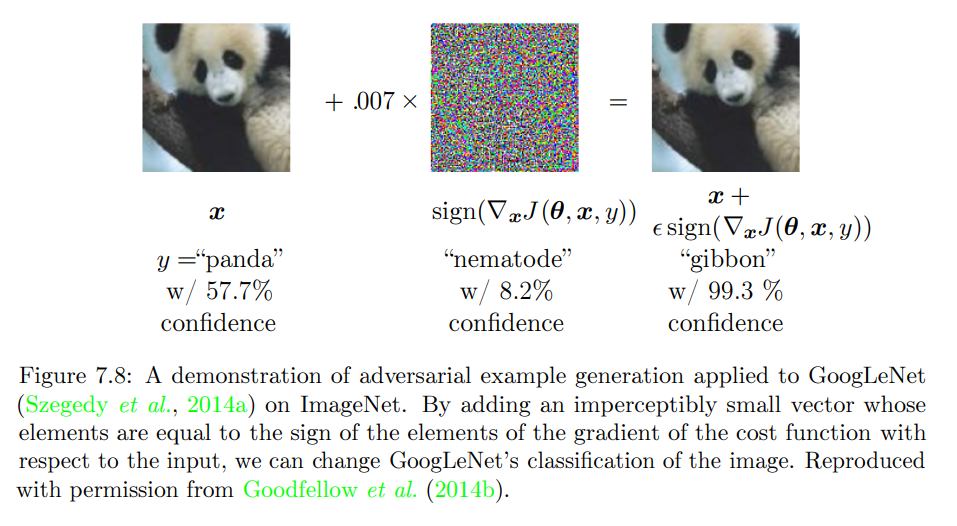
\includegraphics[scale=0.8]{images/Adversarial.png}
\end{center}

